\documentclass[10pt,a4paper]{article}

\usepackage[a4paper, top=2.5cm, bottom=2.5cm, left=2.5cm, right=2.5cm]{geometry}
\usepackage{iftex}
\ifXeTeX
  \usepackage{fontspec}
  \defaultfontfeatures{Ligatures=TeX}
\else
  \usepackage[utf8]{inputenc}
  \usepackage[english]{babel}
\fi

\usepackage{amsmath, amssymb}
\usepackage{booktabs}
\usepackage{array}
\usepackage{tabularx}
\usepackage{setspace}
\usepackage{microtype}
\usepackage{hyperref}
\usepackage{xcolor}
\usepackage{titlesec}
\usepackage{tikz}
\usetikzlibrary{shapes,arrows,positioning}

\titlespacing*{\section}{0pt}{7pt}{3pt}
\titlespacing*{\subsection}{0pt}{5pt}{2pt}

\hypersetup{
    colorlinks=true,
    linkcolor=blue,
    filecolor=magenta,      
    urlcolor=cyan,
    citecolor=blue
}

\setstretch{1.0}
\setlength{\parindent}{1.2em}
\setlength{\parskip}{0pt}
\renewcommand{\arraystretch}{1.1}

% Relax float placement constraints to prevent awkward float pages
\renewcommand{\topfraction}{0.9}
\renewcommand{\bottomfraction}{0.8}
\renewcommand{\textfraction}{0.05}
\renewcommand{\floatpagefraction}{0.85}

\begin{document}

% ==================== TITLE, MEMBERS, ABSTRACT, SECTION 1 ====================

\begin{titlepage}
    \centering

    \vspace*{1.5cm}

    {\Large\bfseries
    UNIVERSITY OF SCIENCE AND TECHNOLOGY OF HANOI (USTH)
    \par}

    \vspace{0.4cm}

    {\large
    MIDTERM PROJECT REPORT
    \par}

    {\normalsize
    Cryptography
    \par}

    \vspace{2cm}

    \rule{\textwidth}{0.6pt}

    \vspace{0.6cm}

    {\LARGE\bfseries
    Design and Implementation of a QR Code-Based
    Digital Certificate Verification System Using RSA
    Digital Signatures
    \par}

    \vspace{0.6cm}

    \rule{\textwidth}{0.6pt}

    \vspace{1.5cm}

    {\large\bfseries
    Group Members
    \par}

    \vspace{0.5cm}

    \renewcommand{\arraystretch}{1.5}
    \begin{tabular}{|c|l|c|}
        \hline
        \textbf{No.} & \textbf{Full Name} & \textbf{Student ID} \\
        \hline
        1 & Nguyễn Khải Điệp & 23BA14051 \\
        \hline
        2 & Doãn Trung Dũng & 23BA14070 \\
        \hline
        3 & Nguyễn Đinh Huyền Mai & 23BA14186 \\
        \hline
        4 & Lương Quỳnh Anh & 23BA14008 \\
        \hline
        5 & Phạm Vũ Khánh & 23BA14148 \\
        \hline
        6 & Đặng Thế Hiệp & 23BA14103 \\
        \hline
        7 & Nguyễn Phương Nam & 23BA14206 \\
        \hline
    \end{tabular}

    \vfill

    {\normalsize
    Academic Year 2026--2027
    \par}

    \vspace{0.5cm}

\end{titlepage}

\begin{abstract}
\noindent Standard QR codes store data in plain text without cryptographic protection, making them easy to tamper with or counterfeit. In this project, we design and implement an offline digital certificate verification prototype in Python using RSA-PSS digital signatures and SHA-256. We first demonstrate the mathematical weakness of Textbook RSA, showing how an attacker can forge valid signatures through modular multiplication without knowing the private key. We then explain how RSA-PSS with randomized salt prevents the direct multiplicative forgery demonstrated in textbook RSA. To improve scanning reliability, we build a multi-stage OpenCV decoding pipeline combining \texttt{QRCodeDetectorAruco} with image preprocessing techniques. In tests with 100 generated RSA-2048 QR codes, our pipeline achieved a 100\% decode rate compared to 80\% for the standard OpenCV detector. Finally, we test five security scenarios and benchmark performance across 1024, 2048, and 3072-bit RSA keys, selecting RSA-2048 as the recommended default.
\end{abstract}

\vspace{-0.15cm}
\section{Introduction}

\subsection{Background and Problem Statement}
Digital certificates are widely used to verify academic degrees, professional licenses, and identity documents. In many daily situations, certificates are printed or displayed as QR codes for fast scanning with mobile devices. However, standard QR codes only serve as an optical data carrier; they provide no built-in security or origin authentication. Anyone can edit certificate data and generate a new QR code that appears completely authentic to an ordinary reader.

To ensure data integrity and detect counterfeiting, digital certificates require cryptographic signatures. In this project, we implement an offline Python Command-Line Interface (CLI) application. The system signs certificate fields using RSA-PSS with SHA-256, embeds the data and signature into a QR code, and allows any verifier with the issuer's public key to verify certificate authenticity without an internet connection.

\subsection{Project Objectives and Scope}
The main goals of this project are:
\begin{enumerate}
    \setlength{\itemsep}{0pt}
    \setlength{\parskip}{0pt}
    \item Convert certificate fields into deterministic JSON format and sign them using RSA-PSS and SHA-256.
    \item Reproduce the multiplicative forgery vulnerability of unpadded Textbook RSA to demonstrate why RSA-PSS is required.
    \item Package signed certificate data into a QR code, and test a compact binary payload format.
    \item Build and evaluate a multi-stage OpenCV QR decoding pipeline to improve scanning success rates.
    \item Evaluate security against tampering and benchmark execution times across different RSA key sizes.
\end{enumerate}

\noindent \textbf{Project Scope and Boundaries:}
\begin{itemize}
    \setlength{\itemsep}{0pt}
    \setlength{\parskip}{0pt}
    \item \textbf{In Scope:} Python CLI prototype; RSA keys (1024, 2048, 3072 bits); canonical JSON serialization; RSA-PSS signing and verification; multi-stage QR decoding; five automated test cases; and performance benchmarks.
    \item \textbf{Out of Scope:} Web application interfaces, central databases, user accounts, and online revocation checking (such as CRL or OCSP). We assume the verifier obtains the public key through a secure channel.
\end{itemize}

% ==================== SECTION 2: THEORETICAL BACKGROUND ====================
\section{Theoretical Background and Weakness Analysis}

\subsection{Cryptographic Primitives and RSA-PSS Mechanics}
Our system integrates four core components, summarized in Table \ref{tab:components}.

\begin{table}[!htbp]
\centering
\caption{Roles of Cryptographic and Encoding Components}
\label{tab:components}
\small
\begin{tabularx}{\textwidth}{>{\raggedright\arraybackslash}p{2.8cm} >{\raggedright\arraybackslash}X}
\toprule
\textbf{Component} & \textbf{Role in the Verification Architecture} \\
\midrule
\textbf{RSA-PSS} & Probabilistic digital signature scheme (RFC 8017 \cite{rfc8017}, FIPS PUB 186-5 \cite{fips186_5}) providing data integrity and issuer authentication relative to a trusted public key. \\
\textbf{SHA-256} & Cryptographic hash function generating a 256-bit collision-resistant message digest (FIPS PUB 180-4 \cite{fips180_4}). \\
\textbf{Private / Public Key} & Asymmetric key pair: private key $(d, n)$ signs data at the issuer; public key $(e, n)$ verifies signatures at the verifier. \\
\textbf{QR Code} & Two-dimensional optical barcode (ISO/IEC 18004 \cite{iso18004}) used solely to transport payload data; provides zero intrinsic security. \\
\bottomrule
\end{tabularx}
\end{table}

RSA key generation produces a public exponent $e = 65537$, a private exponent $d$, and a modulus $n = p \cdot q$ from two large prime numbers $p$ and $q$.

\noindent \textbf{The Mechanics of RSA-PSS and Salt Configuration (RFC 8017 \cite{rfc8017}):}
RSA-PSS (Probabilistic Signature Scheme) provides provable security against chosen-message attacks (EUF-CMA) under standard cryptographic assumptions (Bellare \& Rogaway, 1996 \cite{bellare1996}). Signing proceeds in four steps:
\begin{enumerate}
    \setlength{\itemsep}{0pt}
    \setlength{\parskip}{0pt}
    \item \textbf{Hashing:} The normalized message $M$ is hashed to produce $mHash = \text{SHA256}(M)$ ($hLen = 32$ bytes).
    \item \textbf{Salt Length Configuration:} Our code configures \texttt{salt\_length =} \allowbreak \texttt{padding.PSS.MAX\_LENGTH}. RFC 8017 \cite{rfc8017} defines the maximum salt length as $sLen_{max} = emLen - hLen - 2$, where $emLen = \lceil (modBits - 1)/8 \rceil$. For RSA-2048 with SHA-256, $emLen = 256$ bytes, giving $sLen_{max} = 256 - 32 - 2 = 222$ bytes of random salt.
    \item \textbf{Encoding:} The random salt, $mHash$, and a fixed padding are hashed into $H$. Mask Generation Function 1 (MGF1 with SHA-256) then masks the data block $DB = \text{PS} \parallel \text{0x01} \parallel salt$. The final encoded message is $EM = \text{maskedDB} \parallel H \parallel \text{0xBC}$.
    \item \textbf{Exponentiation:} The encoded block $EM$ is signed with the private key: $s = EM^d \bmod n$.
\end{enumerate}

\subsection{Demonstrating Textbook RSA Weakness (Multiplicative Forgery)}
To explain why padding is necessary, we implemented \texttt{demo\_textbook\_rsa\_forgery} in \texttt{crypto\_utils.py}. In raw Textbook RSA, signing computes $s = m^d \bmod n$ and verification checks $s^e \equiv m \pmod n$. Because modular exponentiation is strictly multiplicative:
\begin{equation}
    \big[(m_1^d \bmod n)(m_2^d \bmod n)\big] \bmod n = (m_1 \cdot m_2)^d \bmod n
\end{equation}
An attacker who collects two valid message-signature pairs $(m_1, s_1)$ and $(m_2, s_2)$ can forge a valid signature $s_3$ for a combined message $m_3 = (m_1 \cdot m_2) \bmod n$ without knowing private key $d$:
\begin{equation}
    s_3 = (s_1 \cdot s_2) \bmod n
\end{equation}

\noindent \textbf{Experimental Verification:} In our demo, we generated valid signatures for $m_1 = 105$ and $m_2 = 200$. We then computed $s_3 = (s_1 \cdot s_2) \bmod n$ and verified it against $m_3 = 21000$. The check returned \texttt{True}. This confirms that raw RSA allows signature forgery through basic arithmetic.

\begin{table}[!htbp]
\centering
\caption{Comparison Between Textbook RSA and RSA-PSS}
\small
\begin{tabularx}{\textwidth}{>{\raggedright\arraybackslash}p{3.3cm} >{\raggedright\arraybackslash}p{4.3cm} >{\raggedright\arraybackslash}X}
\toprule
\textbf{Property} & \textbf{Textbook RSA} & \textbf{RSA-PSS Used Here} \\
\midrule
Randomized encoding & No (deterministic) & Yes; uses fresh random salt \\
Hash-based masking & No (raw integers) & Yes; SHA-256 and MGF1 masking \\
Multiplicative forgery & Vulnerable (demonstrated in test) & Prevented by hash and salt encoding \\
Chosen-message security & Insecure & Provably secure under EUF-CMA \cite{bellare1996} \\
\bottomrule
\end{tabularx}
\end{table}

\noindent \textbf{Why RSA-PSS Prevents This Vulnerability:} RSA-PSS does not sign raw message integers directly. Instead, it applies SHA-256 hashing, randomized salt generation, and MGF1-based encoding before RSA exponentiation. Therefore, the direct multiplicative relationship exploited in textbook RSA cannot be applied in the same way to RSA-PSS signatures.

% ==================== SECTION 3: SYSTEM DESIGN & IMPLEMENTATION ====================
\section{System Design and Implementation}

\subsection{System Architecture and Operational Workflow}
The application provides two operational roles, \textbf{Issuer} and \textbf{Verifier}, within a single interactive Python CLI tool. As summarized in Table \ref{tab:implementation}, the prototype is structured into five dedicated Python modules, while the end-to-end operational workflow is illustrated in Figure \ref{fig:workflow}.

\begin{table}[!htbp]
\centering
\caption{Python Implementation Modules and Their Responsibilities}
\label{tab:implementation}
\small
\begin{tabularx}{\textwidth}{>{\raggedright\arraybackslash}p{3.5cm} X}
\toprule
\textbf{Module} & \textbf{Main Responsibility} \\
\midrule
\texttt{app.py} & Implements the interactive CLI, including RSA key generation, certificate issuance, QR verification, and tampering demonstrations. \\
\texttt{crypto\_utils.py} & Provides RSA key generation, deterministic JSON normalization, RSA-PSS signing and verification, compact payload packaging, and the Textbook RSA forgery demonstration. \\
\texttt{qr\_utils.py} & Handles QR code generation and multi-stage image decoding with OpenCV preprocessing and detector fallback. \\
\texttt{run\_tests.py} & Runs the five security test cases, Textbook RSA forgery demonstration, end-to-end stress test, and RSA performance benchmarks. \\
\texttt{benchmark\_qr\_decoders.py} & Evaluates and compares the standard OpenCV detector with the proposed multi-stage decoding pipeline using 100 generated QR images. \\
\bottomrule
\end{tabularx}
\end{table}

\begin{figure}[!htbp]
\centering
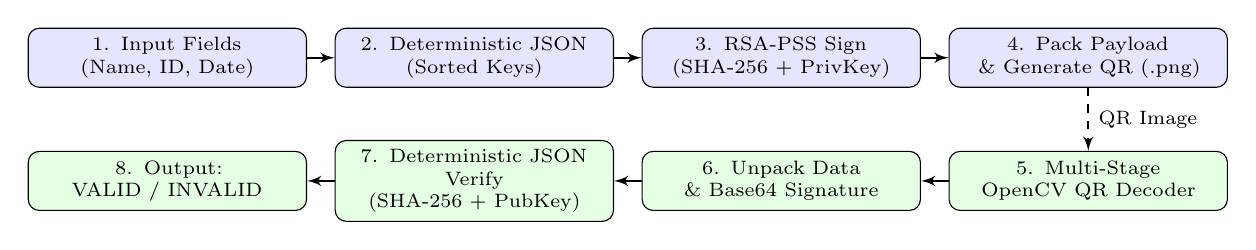
\begin{tikzpicture}[node distance=0.4cm, auto,
    block/.style={rectangle, draw, fill=blue!10, text width=3.3cm, text centered, rounded corners, minimum height=0.75cm, font=\scriptsize},
    block_v/.style={rectangle, draw, fill=green!10, text width=3.3cm, text centered, rounded corners, minimum height=0.75cm, font=\scriptsize},
    line/.style={draw, -latex', thick}]
    
    % Issuer
    \node [block] (in) {1. Input Fields\\(Name, ID, Date)};
    \node [block, right=0.35cm of in] (norm) {2. Deterministic JSON\\(Sorted Keys)};
    \node [block, right=0.35cm of norm] (sign) {3. RSA-PSS Sign\\(SHA-256 + PrivKey)};
    \node [block, right=0.35cm of sign] (qr) {4. Pack Payload\\\& Generate QR (.png)};
    
    % Verifier
    \node [block_v, below=0.8cm of qr] (dec) {5. Multi-Stage\\OpenCV QR Decoder};
    \node [block_v, left=0.35cm of dec] (unp) {6. Unpack Data\\\& Base64 Signature};
    \node [block_v, left=0.35cm of unp] (ver) {7. Deterministic JSON\\Verify \mbox{(SHA-256 + PubKey)}};
    \node [block_v, left=0.35cm of ver] (out) {8. Output:\\VALID / INVALID};
    
    \path [line] (in) -- (norm);
    \path [line] (norm) -- (sign);
    \path [line] (sign) -- (qr);
    \path [line, dashed] (qr) -- node [right, font=\scriptsize] {QR Image} (dec);
    \path [line] (dec) -- (unp);
    \path [line] (unp) -- (ver);
    \path [line] (ver) -- (out);
\end{tikzpicture}
\vspace{-0.2cm}
\caption{End-to-End Certificate Issuance and Verification Workflow.}
\label{fig:workflow}
\end{figure}

The workflow operates in five main steps:
\begin{enumerate}
    \setlength{\itemsep}{0pt}
    \setlength{\parskip}{0pt}
    \item \textbf{Data Normalization:} Given user inputs, \texttt{normalize\_cert\_data()} serializes the dictionary into deterministic JSON with sorted keys (\texttt{sort\_keys=True}) and compact separators (\texttt{separators=(",", ":")}). This guarantees identical byte strings for matching data, avoiding verification errors from formatting variations.
    \item \textbf{Signing:} \texttt{sign\_data()} computes the SHA-256 digest of the normalized JSON string and signs it with RSA-PSS using the issuer's private key ($sLen = 222$ bytes for RSA-2048).
    \item \textbf{QR Packaging:} Certificate fields, Base64 signature, and key ID (\texttt{"EDU-2026"}) are combined into a JSON payload and rendered into a QR code using \texttt{qrcode} (Error Correction Level M).
    \item \textbf{QR Decoding:} \texttt{decode\_qr\_image()} extracts the payload from the image using our multi-stage pipeline.
    \item \textbf{Verification:} \texttt{unpack\_qr\_payload()} parses the data and signature. Then \texttt{verify\_signature()} re-normalizes the certificate dictionary and checks the signature against the trusted public key.
\end{enumerate}

\subsection{Robust Multi-Stage QR Decoding Pipeline}
Dense QR codes (such as Version 17) can fail to decode using OpenCV's standard detector. To solve this, we implemented a cascading fallback pipeline in \texttt{qr\_utils.py}:
\begin{itemize}
    \setlength{\itemsep}{0pt}
    \setlength{\parskip}{0pt}
    \item \textbf{Detector fallback:} Tries OpenCV 4.7+ \texttt{cv2.}\allowbreak\texttt{QRCodeDetector}\allowbreak\texttt{Aruco()} first, falling back to \texttt{QRCodeDetector()} if unavailable.
    \item \textbf{Preprocessing fallbacks:} Progressively applies color BGR decoding, grayscale conversion, white quiet-zone padding (following ISO/IEC 18004 \cite{iso18004}), Otsu thresholding, and nearest-neighbor scaling (\texttt{INTER\_NEAREST}).
\end{itemize}

\noindent \textbf{Decoder Benchmark Comparison:} We tested both methods on 100 generated RSA-2048 QR images using \texttt{benchmark\_qr\_decoders.py}. Each image contained the same certificate details with a fresh RSA-PSS signature and randomized salt. All images were unmodified software-generated QR Version 17 PNGs ($744 \times 744$ pixels, EC=M).
\begin{center}
\small
\textbf{Measured Decoder Performance (100 Test Images)}\par
\begin{tabular}{l c c c}
\toprule
\textbf{Method} & \textbf{Success Rate} & \textbf{Failures} & \textbf{Mean Time (ms/image)} \\
\midrule
OpenCV \texttt{QRCodeDetector()} baseline & 80/100 (80\%) & 20 & 77.71 \\
Multi-stage pipeline & 100/100 (100\%) & 0 & 98.50 \\
\bottomrule
\end{tabular}
\end{center}
\noindent On this dataset, the multi-stage pipeline eliminated all 20 baseline failures with a modest 27\% increase in average decoding latency (98.50 ms vs. 77.71 ms). These results are limited to software-generated QR images and do not establish equivalent performance under real-world camera conditions, such as varying lighting, perspective distortion, or motion blur.

\subsection{Payload Optimization and Security Considerations}
\begin{itemize}
    \setlength{\itemsep}{0pt}
    \setlength{\parskip}{0pt}
    \item \textbf{Payload Optimization:} An RSA-2048 signature produces 256 raw bytes (344 Base64 characters). Our compact format compresses the metadata dictionary using zlib, prepends a 2-byte length header, and appends the raw signature bytes before Base64 encoding. This reduces payload size from 488 bytes to 470 bytes (a 3.69\% reduction), though both fit within QR Version 17. Standard readable JSON remains the default for transparency.
    \item \textbf{Key Storage:} Sample private keys are stored unencrypted for demonstration purposes. In production environments, private keys must be protected with passphrases (e.g., AES-256) or managed inside Hardware Security Modules (HSMs).
\end{itemize}

% ==================== SECTION 4: EVALUATION & CONCLUSION ====================
\section{Experimental Evaluation and Conclusion}

\subsection{Security and Tamper Detection Test Cases}
We evaluated system security using five automated scenarios in \texttt{run\_tests.py} (Table \ref{tab:testcases}).

\begin{table}[!htbp]
\centering
\caption{Security and Tamper Detection Test Scenarios}
\label{tab:testcases}
\small
\setlength{\tabcolsep}{4pt}
\begin{tabularx}{\textwidth}{l >{\raggedright\arraybackslash}X >{\raggedright\arraybackslash}X >{\raggedright\arraybackslash}p{1.9cm} >{\raggedright\arraybackslash}p{2.1cm} c}
\toprule
\shortstack{\textbf{Test ID}} & \shortstack{\textbf{Objective /}\\\textbf{Scenario}} & \shortstack{\textbf{Input}\\\textbf{Condition}} & \shortstack{\textbf{Expected}\\\textbf{Result}} & \shortstack{\textbf{Actual}\\\textbf{Result}} & \textbf{Status} \\
\midrule
\textbf{TC-01} & Valid certificate issuance & Authentic QR + Matching Public Key & Valid Signature & \textbf{Valid Signature} & \textbf{PASS} \\
\textbf{TC-02} & Detect data tampering & Name altered to \texttt{Nguyen Van B (Fake)} & Invalid Signature & \textbf{Invalid Signature} & \textbf{PASS} \\
\textbf{TC-03} & Detect signature tampering & First 10 Base64 signature characters edited & Invalid Signature & \textbf{Invalid Signature} & \textbf{PASS} \\
\textbf{TC-04} & Verify issuer authenticity & Authentic QR + Wrong RSA-2048 Public Key & Invalid Signature & \textbf{Invalid Signature} & \textbf{PASS} \\
\textbf{TC-05} & Error handling on bad input & Corrupted / non-image byte stream & Graceful error & \textbf{Cannot decode QR} & \textbf{PASS} \\
\bottomrule
\end{tabularx}
\end{table}

\noindent All modified payloads and mismatched keys were successfully detected and rejected. Copying an intact QR code is not detected by design, as the QR code itself carries no device-bound credentials.

\subsection{Automated 100-Run Stress Test and Performance Benchmark}
In an automated stress test, the system performed 100 consecutive iterations of certificate generation, signing, QR encoding, decoding, and verification. The run completed with a 100/100 success rate in 26.80 seconds (recorded in \texttt{sample\_qrs/decoder\_eval/run\_tests\_output.txt}).

We also measured signing and verification times across 1024, 2048, and 3072-bit keys (averaged over 30 runs using \texttt{time.perf\_counter()} on Windows 11, Python 3.14.2, Cryptography 50.0.2, OpenCV 4.13.0):

\begin{table}[!htbp]
\centering
\caption{Benchmark Results Across RSA Key Sizes (Averaged Over 30 Runs)}
\label{tab:benchmark}
\small
\begin{tabular}{l c c c c}
\toprule
\textbf{Key Size} & \textbf{Signing Time (ms)} & \textbf{Verification Time (ms)} & \textbf{Payload (JSON / Compact)} & \textbf{QR Version} \\
\midrule
RSA-1024 & 13.093 & 0.032 & 316 / 298 B & 13 \\
RSA-2048 & 69.990 & 0.163 & 488 / 470 B & 17 \\
RSA-3072 & 127.758 & 0.064 & 656 / 642 B & 20 \\
\bottomrule
\end{tabular}
\end{table}

\noindent Signing involves large modular exponentiation with the private key exponent $d$, so signing time increases with larger key sizes (13.09 ms for RSA-1024 to 127.76 ms for RSA-3072). In contrast, verification uses the small public exponent $e = 65537$, making verification extremely fast (under 0.2 ms across all key sizes). RSA-2048 offers the best balance between security ($\approx$ 112-bit security strength) and practical performance, meeting modern digital signature recommendations \cite{fips186_5}.

\subsection{Limitations and Conclusion}
\textbf{Limitations:} The system assumes that the verifier already has an authentic copy of the issuer's public key. The signature guarantees data integrity, but it cannot prevent an attacker from copying and replaying an intact QR code. Real-time key revocation is also outside the scope of this offline prototype.

\noindent \textbf{Conclusion:} This project demonstrates an offline QR certificate verification system using RSA-PSS and SHA-256. The system reliably detects data tampering, signature alterations, and unauthorized keys while maintaining fast, sub-millisecond verification.

\begin{thebibliography}{5}
\setlength{\itemsep}{0pt}
\setlength{\parskip}{0pt}
\small
\bibitem{rfc8017} K. Moriarty, B. Kaliski, J. Jonsson, and A. Rusch, \textit{PKCS \#1: RSA Cryptography Specifications Version 2.2} (RFC 8017), Internet Engineering Task Force (IETF), 2016.
\bibitem{fips180_4} National Institute of Standards and Technology (NIST), \textit{Secure Hash Standard (SHS)}, FIPS PUB 180-4, U.S. Department of Commerce, 2015.
\bibitem{fips186_5} National Institute of Standards and Technology (NIST), \textit{Digital Signature Standard (DSS)}, FIPS PUB 186-5, U.S. Department of Commerce, 2023.
\bibitem{iso18004} International Organization for Standardization, \textit{Information technology --- Automatic identification and data capture techniques --- QR Code bar code symbology specification} (ISO/IEC 18004:2015), 2015.
\bibitem{bellare1996} M. Bellare and P. Rogaway, ``The Exact Security of Digital Signatures: How to Sign with RSA and Rabin,'' in \textit{Advances in Cryptology --- EUROCRYPT '96}, LNCS 1070, pp. 399--416, 1996.
\end{thebibliography}

\end{document}
